\chapter{Einleitung}
\label{cha:einleitung}

In dieser Dokumentation wird die Entwicklung einer App im Rahmen des Anwendungsfaches Mobile Application Lab an der Universität Ulm und die dadurch erstellte App in Form einer Quartett App vorgestellt.

% Abschnitt: Problemstellung
\section{Motivation und Problemstellung}
\label{sec:einleitung:problemstellung}

Die Problemstellung wurde uns im Rahmen dieses Projektes schon gegeben, da wir uns auf die Entwicklung einer Quartett App für Smartphones konzentrieren sollten. Das Prinzip des beliebten Kartenspiels soll für ein Smartphone entwickelt werden und so zu jeder Zeit und an jedem Ort auch ganz ohne physiche Karten spielbar sein.

Beim Anschauen des aktuellen Marktes für Quartett Apps fällt schnell die Vielzahl an verschiedenen Apps auf. Diese erweisen nach genauerem Betrachten jedoch erhebliche Mängel auf. So sind manche von ihnen sehr veraltet und funktionieren nicht mehr richtig auf neueren Smartphone Modellen. Auch entsprechen diese inhaltlich nicht unseren Vorstellungen von einer guten Quartett App. Sie sind sehr beschränkt, was die verschiedenen Spielmodi angeht und beschräken sich meistens auf ein einziges Kartendeck oder Decks aus einem Themengebiet.

% Abschnitt: Zielsetzung
\section{Zielsetzung}
\label{sec:einleitung:zielsetzung}

Da auf dem Markt eine Nachfrage besteht wollen wir diese ausnutzen und eine eigene Quartett Anwendung erstellen. Diese wollen wir auf Basis von Android und Java entwickeln. Dabei geht es uns primär darum, den Umgang mit den neuen Techniken zu erlernen und eine Grunderfahrung im Programmieren von Android Anwendungen zu erlangen, sodass wir diese nach Abschließen des Projektes beherrschen können.

Inhaltlich möchten wir eine Quartett App entwickeln, die sich als Singleplayer wie ein richtiges Quartett spielen lässt. Sie soll verschiedene Spielmodi haben, welche frei konfigurierbar sein sollen. Zudem soll die Auswahl an Decks breit gefächert sein, was durch einen Deckcreator und einer Onlinefunktion zum Up- und Downloaden realisiert werden soll. Der Anwendung soll zudem die Möglichkeit bieten, alle Karten anzugucken und laufende Spiele zu unterbrechen. Dabei soll die App benutzerfreundlich sein und schön aussehen, sowie auf den neusten aber auch auf älteren Android Smartphones lauffähig sein.

% Abschnitt: Struktur der Arbeit
\section{Struktur der Arbeit}
\label{sec:einleitung:struktur}

In dieser Dokumentation werden zuerst einmal grundlegend die Quartett Spielregeln erklärt sowie Android vorgestellt und unsere verwendeten Frameworks präsentiert. Den Hauptteil bildet die Implementierung, welche unsere App im Allgemeinen und mit ihren Besonderheiten vorstellt. Außerdem wird darin unsere Architektur gezeigt und wir erleutern Schwierigkeiten, die wir während der Implementierungsphase hatten. Abschließend gibt es einen Anforderungsabgleich und einen Ausblick auf die Zukunft des Projektes.\\

\begin{figure}[htp]
	\centering
  	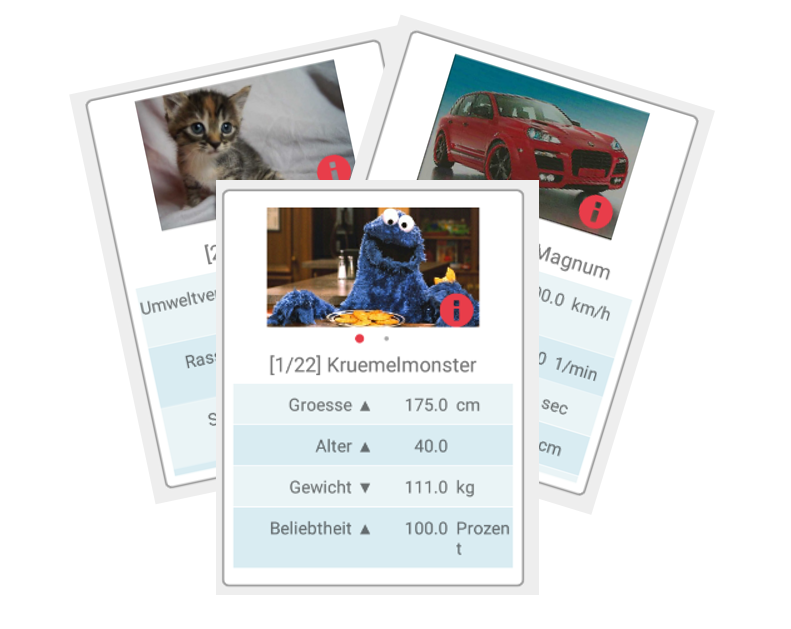
\includegraphics[width=0.4\textwidth]{img/quartett42_logo.png}
	\caption{Quartett42 Logo}
	\label{figure:quartett42logo}
\end{figure}
